\section{Theory of Operations}

\subsection{Introduction}
The UART module is designed for full–duplex asynchronous serial communication.
It implements independent transmitter (TX) and receiver (RX) paths that operate concurrently.
Both paths include configurable settings for baud rate, data length, and parity.
In addition, each side incorporates an internal FIFO buffer to decouple external data handling
from the serial transmission or reception. Figure~\ref{fig:uart_blockdiagram}
shows a high-level block diagram and Figure~\ref{fig:frame_formats} shows a diagram of the UART protocol frame format.

\begin{figure}[H]
  \centering
  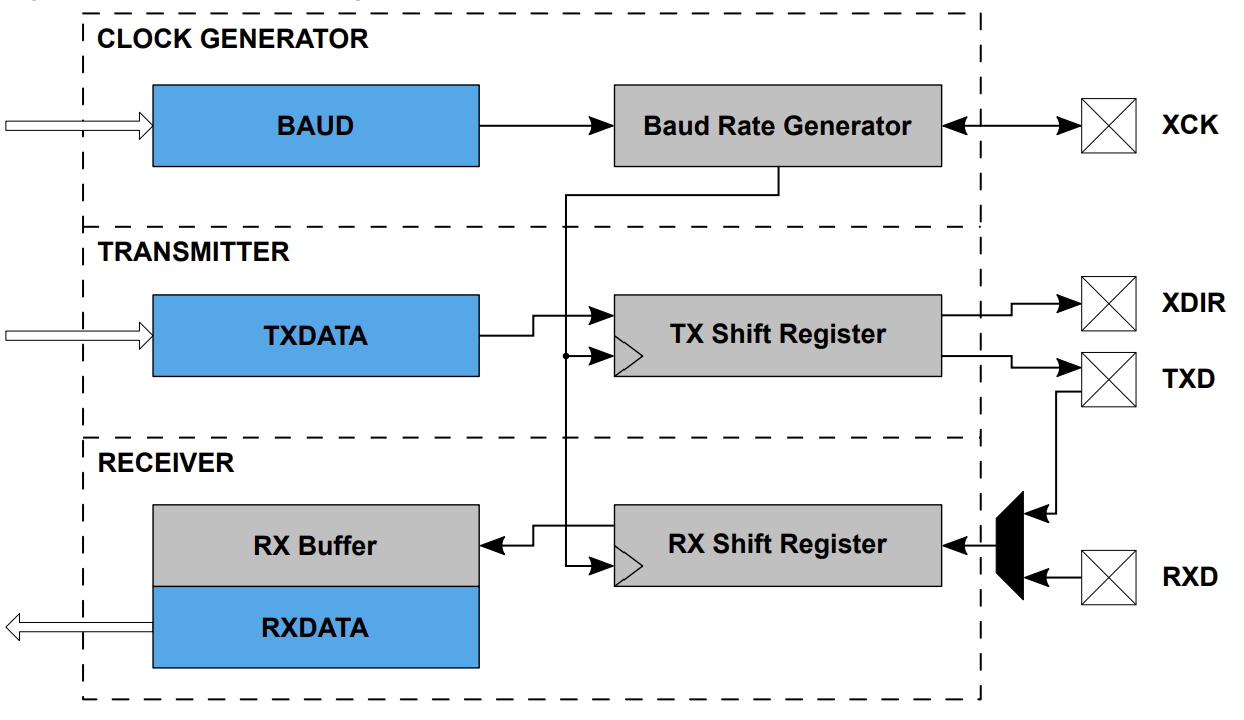
\includegraphics[width=0.85\textwidth]{images/uart_block_diagram.png}
  \caption{UART Block Diagram}
  \label{fig:uart_blockdiagram}
\end{figure}

\begin{figure}[H]
    \centering
    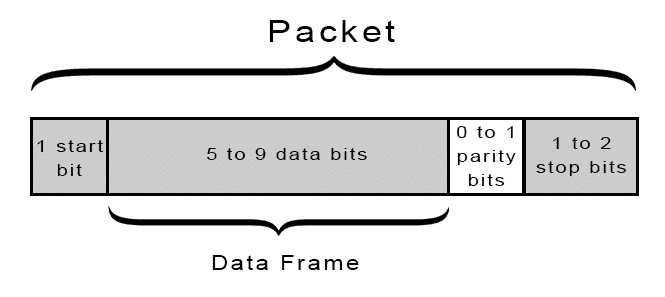
\includegraphics[width=0.85\textwidth]{images/frame_format.png}
    \caption{Frame Formats}
    \label{fig:frame_formats}
\end{figure}

\subsection{State Machine}
The UART module has the following states in its state machines:
\begin{itemize}
    \item \texttt{Idle}: Waiting for new data and/or baud update.
    \item \texttt{BaudUpdating}: Waiting for the baud rate generator to compute \texttt{clocksPerBit}.
    \item \texttt{Start}: Driving the start bit.
    \item \texttt{Data}: Shifting out the data bits.
    \item \texttt{Parity}: (Optional) Transmitting the parity bit.
    \item \texttt{Stop}: Driving the stop bit before returning to \texttt{Idle}.
\end{itemize}

\begin{figure}[H]
  \centering
  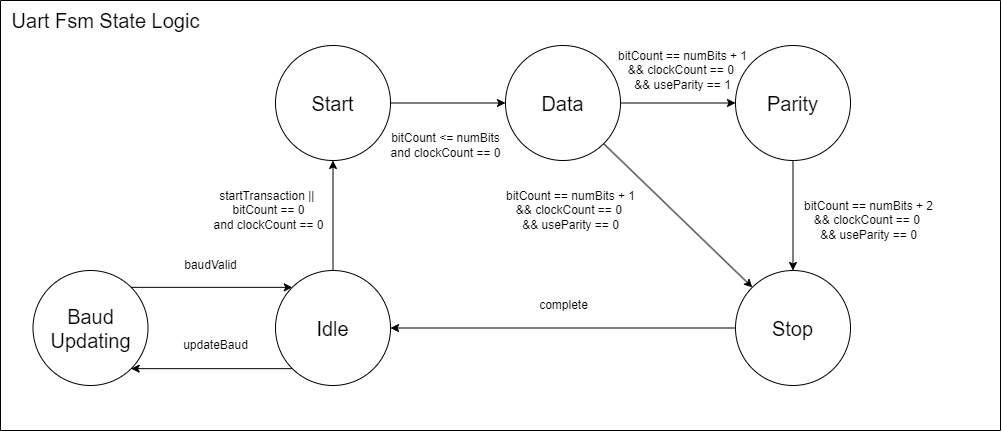
\includegraphics[width=0.85\textwidth]{images/uartfsm.drawio.png}
  \caption{UART State Machine}
  \label{fig:uartfsm}
\end{figure}

\subsection{Clocking and Synchronization}
All logic is synchronous to the APB clock (\texttt{PCLK}). The \texttt{rx} pin is passed through \textit{syncDepth} flip-flops to reduce metastability. The TX path uses the same clock domain and counters to generate appropriate bit timing.

\subsection{Data Flow}
\textbf{Transmit}:
\begin{itemize}
    \item Software writes data into the \texttt{TX\_DATA\_IN} register which automatically write into the FIFO.
    \item A send trigger (e.g., pulsing \texttt{TX\_LOAD}) pops all data from the FIFO in the order it came in one after the other.
\end{itemize}

\noindent
\textbf{Receive}:
\begin{enumerate}
  \item The RX logic waits for a start bit (transition from high to low).
  \item Data bits are shifted in at intervals determined by \texttt{RX\_CLOCKSPERBIT}, followed by optional parity and the stop bit.
  \item Completed bytes are pushed into the RX FIFO; software reads them via \texttt{RX\_DATA} or \texttt{RX\_DATAPEEK} in the order they arrived.
\end{enumerate}
